\documentclass{article}
\usepackage{iclr2027_conference,times}
\input{math_commands.tex}
\usepackage[T1]{fontenc}
\usepackage{amsmath,amssymb,booktabs,graphicx,microtype,multirow}
\usepackage[hidelinks]{hyperref}
\usepackage{url}
\newcommand{\AlfPlanned}{384}
\newcommand{\SwPlanned}{57}
\newcommand{\AlfGroups}{96}
\newcommand{\SwGroups}{25}
\newcommand{\EligibleTotal}{406}
\newcommand{\AlfEligible}{355}
\newcommand{\SwEligible}{51}
\newcommand{\AlfEarly}{29}
\newcommand{\SwEarly}{6}
\newcommand{\ResultDigest}{f10ee7cf00106313b2d66e34326e78f13f3e49b44f13774d955802599e1573e5}


\title{Selection Is Not Evaluation:\\Independent Continuations for Runtime Intervention in Language Agents}

\author{Anonymous authors}

\begin{document}
\maketitle

\begin{abstract}
Selecting a runtime intervention and evaluating it on the same stochastic continuation credits favorable branch noise. We generate two independently seeded continuations for every action from a shared prefix. The same draws separate the action that is chosen from the outcome that scores it and, before any controller is fitted, read how much room a decision point and an action menu leave. On 384 identity-disjoint ALFWorld tasks the same-draw maximum overstates cross-draw value by 15.36 percentage points (floorplan-bootstrap 95\% interval [12.46, 18.30]), and does not exceed a within-task exchangeable-label reference of 17.26 points on eligible prefixes. At a hash-assigned early step with four fixed messages, a selector reading one independent draw of every action reaches 50.28\% against 51.69\% for the best arm in hindsight, replanning, so no prefix-conditional rule can win there. Moving the decision to the first public failure signal and separating repair depth from content lifts it to 50.80\% against 49.09\%. On 593 further tasks a controller that chooses its action on one development draw and values it on another captures 79 percent of the room so created on triggered prefixes and leads every matched comparator, by 1.26 points over continuation across all planned tasks and by 1.94 over the best fixed repair.

\end{abstract}

\section{Introduction}

A language agent can be warned, asked to replan, or rolled back when a trajectory appears to be failing. None of these repairs is free. A warning can displace useful context, a new plan can abandon partial progress, and a rollback can undo a correct action. A runtime controller must therefore answer a treatment-choice question: which action, including no intervention, has the highest expected utility from the current prefix?

The evaluation is easy to bias. Suppose an experiment restores one agent prefix, samples several intervention branches, and chooses the branch with the best observed outcome. Scoring that choice on the same sampled branches measures a realized maximum. It credits the selection rule for favorable continuation noise. The problem is acute in binary-success environments, where one lucky branch can turn an otherwise tied action menu into an apparent rescue. Repeating the task under a different seed is not enough if the repeated outcome is again used both to choose and to score the action.

This distinction is separate from two established ideas. First, outcome regression and direct treatment-effect regression are alternative target parameterizations for heterogeneous treatment effects \citep{kunzel2019metalearners}. Second, separating selection from evaluation is a general remedy for maximization bias and adaptive reuse \citep{vanhasselt2010double,dwork2015generalization}. We apply both distinctions to intervention policies for language agents. The closest same-prefix study, \citet{zhang2026calibration}, evaluates the main controller with one realized branch per action and repeats three actions twice on 24 shallow ALFWorld prefixes as a stability check. \citet{jiang2026cota} compare concrete candidate actions with a learned advisor, but their actor history, action support, intervention frequency, and compute differ from the fixed repair menu studied here.

We use two independently seeded continuations for each of four actions from a shared prefix. Any policy fitted on separate development tasks is evaluated on both draws. For an outcome-informed oracle diagnostic, the action selected on one draw is evaluated on the other. This yields a symmetric, pathwise nonnegative gap between the observed maximum and the independent-draw value of the selected action. The gap measures how much a same-outcome analysis can overstate deployable utility on the sampled task frame. It does not establish that any learned intervention helps.

The controller comparison holds the development records, observable prefix features, four task-group folds, 200-tree capacity, margin grid, and action menu fixed. One forest predicts four arm outcomes. A second predicts three signed benefits relative to continuation,
\begin{equation}
\Delta_a(x)=\mathbb{E}[Y_a-Y_0\mid X=x],\qquad a\in\{1,2,3\}.
\end{equation}
Both controllers can choose \textsc{Continue}. The candidate set also contains the development-best fixed arm and the strongest runnable policy from the existing arm-outcome family. All predictions were committed before confirmation arm outcomes were generated.

The confirmation panel contains \AlfPlanned{} ALFWorld tasks balanced over six task types and grouped by \AlfGroups{} floorplans. Their goal directories are absent from the supplied prior configuration and outcome-exposure packet. A secondary panel contains \SwPlanned{} previously reserved ScienceWorld official-test variations that were not present in that packet. ALFWorld is the target population because development evidence selected it; ScienceWorld is a boundary analysis, not a second claim of broad generality. We report the complete primary family, every frozen policy, costs, early-terminal tasks, and the adverse historical evidence.

The paper makes three contributions. It gives a repeated-branch protocol and a simple diagnostic that prevents a realized action maximum from being reported as policy value. It provides a controlled target-parameterization comparison between direct signed-benefit and arm-outcome forests, with explicit no-intervention and fixed-arm fallbacks. It also releases a pre-outcome configuration, prediction freeze, bounded compute ledger, full result census, and scripts that regenerate every table and figure. The empirical conclusions are stated in Section~\ref{sec:results}; they are not widened beyond the frozen tests.

\section{Evaluating a runtime intervention}
\label{sec:estimand}

\subsection{Policy value after a shared prefix}

Let $X_i$ be the observable prefix for task $i$ at its assigned checkpoint and let $E_i=1$ when the episode ends before that checkpoint. The action set is $\mathcal{A}=\{0,\ldots,K\}$, where $0$ means continue without an injected message. A stochastic continuation under action $a$ produces binary task success $Y_{ia}\in\{0,1\}$ with conditional mean $\mu_a(x)=\mathbb{E}[Y_{ia}\mid X_i=x]$. A prefix-only policy $\pi(a\mid x)$ acts only on eligible prefixes, so the reported task-level value is a mixture,
\begin{equation}
V(\pi)=\mathbb{P}(E=1)\,\mathbb{E}\!\left[Y^{\mathrm{early}}\mid E=1\right]
+\mathbb{P}(E=0)\,\mathbb{E}_{X\mid E=0}\!\left[\sum_{a\in\mathcal{A}}\pi(a\mid X)\mu_a(X)\right].
\label{eq:policy-value}
\end{equation}
Early-terminal tasks contribute their observed terminal outcome to every policy, so they cancel from every contrast and enter only the denominator. The expectation includes continuation randomness. A single fresh draw per task is already an unbiased estimate of $V(\pi)$ for a policy committed before that draw; the bias studied next arises only when the action is chosen using the outcome that then scores it. A controller that always intervenes can have lower value than continuation even when it correctly detects a difficult prefix. Detection quality and treatment choice are different estimands \citep{vasudev2026failure}.

Our simulated environments permit a repeated-branch design. From the same serialized state, we generate two draws $Y_{ia}^{(0)}$ and $Y_{ia}^{(1)}$ for every action. The request seeds are independent deterministic hashes of task, draw, action, and request index. Full-state hashes validate restoration before the first suffix call. The actor sees only the common public prefix, the assigned message, and subsequent observations.

\subsection{The same-draw optimism diagnostic}

Define $\widehat a_i^{(r)}=\arg\max_a Y_{ia}^{(r)}$, resolving ties by the lowest action index, so continuation wins every tie it enters and the lowest-indexed successful intervention wins otherwise. A same-draw analysis scores this outcome-informed choice as $\max_aY_{ia}^{(r)}$. Cross-draw evaluation instead scores the selected action on the other draw. We use the symmetric gap
\begin{equation}
G_i=\frac{1}{2}\!\left[
\max_aY_{ia}^{(0)}-Y_{i,\widehat a_i^{(1)}}^{(0)}+
\max_aY_{ia}^{(1)}-Y_{i,\widehat a_i^{(0)}}^{(1)}
\right].
\label{eq:gap}
\end{equation}

\textbf{Proposition 1.} $G_i\geq0$ for every realized pair of action-outcome vectors. If the two action-outcome vectors are independent and identically distributed conditional on $X_i$, then $\mathbb{E}[G_i\mid X_i]$ equals the expected same-draw maximum minus the independent-draw value of the action chosen on that draw.

The pathwise statement follows because each maximum is at least the outcome of the action selected on the other draw; it needs no distributional assumption. Conditional independence is what factors the cross-draw term into the value of the selection rule on a fresh continuation, and identical distribution is what makes the two orderings interchangeable. Without independence the identity fails: two perfectly dependent draws give $G_i\equiv0$ while the expected same-draw maximum still exceeds the independent-draw value whenever continuation outcomes are stochastic. With $R>2$ draws the same statement holds for the average of $G$ over ordered draw pairs. A positive $G_i$ can arise from unstable binary outcomes even when all actions have the same conditional mean. Because $G_i\geq0$ pathwise, a sign-flip null is degenerate for it: every group sum is non-negative, so the test can only reject the sharp null of deterministic continuations. We therefore treat $G$ as an estimation diagnostic and read it against a within-task reference distribution that permutes the action and draw labels of the eight recorded outcomes, which fixes the continuation noise level and removes any action structure. Appendix~\ref{app:proof} gives the derivation and tie cases.

Figure~\ref{fig:design} shows the information boundary. Frozen policies use the prefix only. The outcome-informed selector exists solely to quantify same-draw optimism; it is not a deployable method or a training label for the confirmation policies.

\begin{figure}[t]
\centering
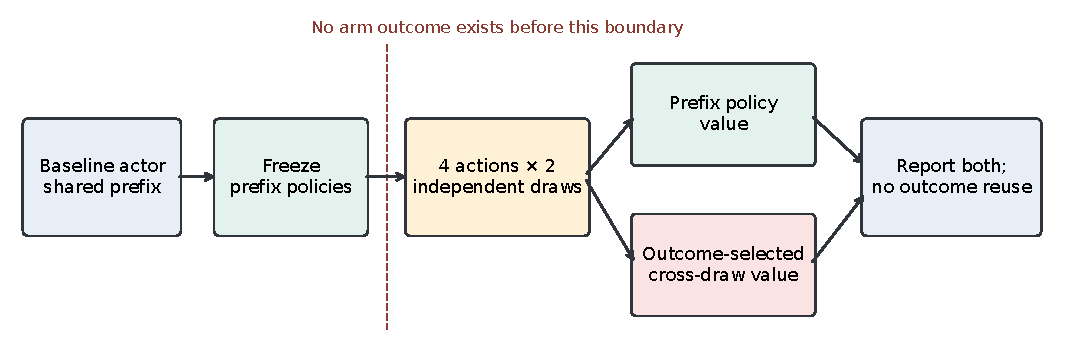
\includegraphics[width=\linewidth]{figures/design.pdf}
\caption{Repeated-branch confirmation. A baseline actor creates a checkpoint. Every eligible prefix is restored for four actions and two independently seeded draws. Prefix-only controller predictions are frozen before any of these arm outcomes. Outcome-informed action choice on draw 0 is scored on draw 1 and vice versa.}
\label{fig:design}
\end{figure}

\section{Controllers with a continuation option}
\label{sec:controllers}

\subsection{Matched target parameterizations}

The repeated arm-outcome learner fits a multi-output random forest \citep{breiman2001random} to
\begin{equation}
\bar Y_{ia}=\frac{Y_{ia}^{(0)}+Y_{ia}^{(1)}}{2},\qquad a\in\mathcal A.
\end{equation}
At prediction time it compares four estimated outcome means. The direct learner uses the same records but fits three outputs,
\begin{equation}
\bar D_{ia}=\frac{1}{2}\sum_{r=0}^{1}\left(Y_{ia}^{(r)}-Y_{i0}^{(r)}\right),
\qquad a\in\{1,2,3\}.
\end{equation}
Its continuation score is fixed at zero. Thus the two learners differ in the response target while retaining the same action menu and predictor class. The comparison does not assume that direct effect regression is uniformly preferable; such an ordering is absent even in standard heterogeneous-effect settings \citep{kunzel2019metalearners}.

Both learners receive public information available at the fork: environment identifier, checkpoint index, counts of invalid or inadmissible actions, reward and usage summaries, action repetition signals, recent observations and actions, and recent prefix text. Hidden state hashes and reversibility metadata are excluded. Numeric fields are vectorized directly. Recent text uses a 512-term TF--IDF vocabulary fitted within each training fold and at most 16 truncated-SVD components.

Model selection uses four shuffled whole-task folds with seed 260908. Each candidate has 200 trees, minimum leaf size 5 or 10, and a continuation margin in $\{0,0.05,0.10\}$. Vocabulary and projection fitting occur inside each fold. Out-of-fold utility selects the configuration, and lower intervention rate breaks utility ties. The final forests are refit on all admitted development tasks. Source and target hashes, fold identities, feature schemas, library versions, and every candidate score are stored in the model manifests.

\subsection{Cross-draw selection inside the controller}
\label{sec:crossdraw}

A deployed controller also maximizes. It compares estimates $\widehat\Delta_a(x)$ and fires the arm attaining their maximum, so the score that the margin test sees is a realized maximum over noisy estimates and inherits the bias of Section~\ref{sec:estimand} at the estimation level rather than the outcome level. The repeated-branch design already supplies the remedy it needs. We fit one signed-benefit forest per development draw, $\widehat\Delta^{(0)}$ and $\widehat\Delta^{(1)}$, on identical features, folds, and capacity. The arm is chosen on one draw and valued on the other,
\begin{equation}
\widehat a^{(r)}(x)=\arg\max_a\widehat\Delta^{(r)}_a(x),
\qquad
S(x)=\tfrac12\!\left[\widehat\Delta^{(1)}_{\widehat a^{(0)}(x)}(x)+\widehat\Delta^{(0)}_{\widehat a^{(1)}(x)}(x)\right],
\label{eq:crossdraw}
\end{equation}
and the controller intervenes only when the two draws agree on the arm and $S(x)$ exceeds the continuation margin. Equation~\ref{eq:crossdraw} is Equation~\ref{eq:gap} moved from the evaluator to the controller: the same symmetric construction, applied to estimates rather than outcomes, and the same requirement that the quantity used to choose never be the quantity used to value. Agreement is a stability requirement, not a confidence statement; it declines to act when the two draws disagree about which repair the prefix calls for.

Model selection faces the same problem once more, because the development grid is scored and then maximized on the same folds. We therefore report a nested out-of-fold utility that selects the leaf and margin inside each training fold and scores the resulting rule on the held-out fold, alongside the plain out-of-fold utility used by the frozen candidate rule.

\subsection{Fallbacks and the comparator}

The policy set contains five distinct decisions at confirmation time. \textsc{Continue} always chooses $a=0$. \textsc{Best fixed} chooses the development-best arm, which is replanning ($a=2$) in both environments. \textsc{Direct} uses the signed-benefit learner. \textsc{Arm outcome} uses the two-draw outcome forest and isolates response parameterization. \textsc{Matched comparator} is the strongest runnable member of the existing arm-outcome family by development out-of-fold utility. It is \textsc{Single-1}, an otherwise matched forest fitted to one predesignated outcome draw.

The operational candidate set is $\{\textsc{Continue},\textsc{Best fixed},\textsc{Direct},\textsc{Matched comparator}\}$. Its development-only selection uses the same utility and tie rule. The selected policy is reported as \textsc{Safe selected} even when it is a baseline or an existing learner. In both environments the frozen selection chose \textsc{Single-1}. Calling this rule safe means only that it can decline intervention and was selected without confirmation outcomes; it is not a safety guarantee.

\begin{table}[t]
\caption{Controlled comparison and frozen action menu}
\label{tab:design}
\centering
\small
\begin{tabular}{@{}lll@{}}
\toprule
Component & Arm-outcome forest & Direct signed-benefit forest \\
\midrule
Development rows & Same two-draw task blocks & Same two-draw task blocks \\
Features and text & Shared prefix transform & Shared prefix transform \\
Folds and capacity & 4 groups; 200 trees & 4 groups; 200 trees \\
Leaf and margin grid & $\{5,10\}$; $\{0,.05,.10\}$ & $\{5,10\}$; $\{0,.05,.10\}$ \\
Response & $(\bar Y_0,\ldots,\bar Y_3)$ & $(\bar D_1,\bar D_2,\bar D_3)$ \\
No-intervention action & $a=0$ & zero-benefit reference \\
\midrule
$a=0$ & \multicolumn{2}{l}{Continue with no injected message} \\
$a=1$ & \multicolumn{2}{l}{Check goal, observation, and previous action} \\
$a=2$ & \multicolumn{2}{l}{Construct and execute a fresh concise plan} \\
$a=3$ & \multicolumn{2}{l}{Undo the previous action, then replan; matched decision budget} \\
\bottomrule
\end{tabular}
\end{table}

\section{Independent confirmation design}
\label{sec:design}

\subsection{Actor and interventions}

The actor is Qwen3-8B at revision \texttt{b968826d9c46dd6066d109eabc6255188de91218} \citep{yang2025qwen3}. It receives a grounded ReAct-style prompt \citep{yao2023react}: one short thought followed by an exact valid action. Thinking mode is disabled. Generation uses temperature 0.7, top-$p$ 0.9, at most 256 output tokens, and a 32,768-token context. Serving uses deterministic-inference mode in a content-addressed SGLang container. This setting fixes the sampling implementation for the study; seeded language-model generation is not claimed to be universally invariant across hardware or serving systems \citep{bjarnason2026randomness}.

ALFWorld episodes have a 50-action limit and checkpoints at step 4 or 8 \citep{shridhar2021alfworld}. ScienceWorld episodes have a 100-action limit and checkpoints at step 8 or 16 \citep{wang2022scienceworld}. A hash of each task identity assigns the checkpoint before generation. Action 3 restores the state before the last executed action and reduces the suffix limit by one. The other arms restore the checkpoint state. This gives every arm the same total decision budget. The intervention message is inserted once at the restored step and remains in history; no controller sees future state or outcome fields.

Each task first receives one baseline episode. A task that terminates before its assigned checkpoint has no intervention decision. Its observed terminal success is assigned to every policy and all contrasts and optimism terms are zero. For every eligible task, two fresh continuation arms are generated rather than copying the suffix of the baseline episode. This matters because the baseline trajectory helped define the prefix.

\subsection{Panels and exposure boundary}

The primary panel has \AlfPlanned{} ALFWorld tasks, 64 from each of the benchmark's six task types. Tasks come from the ALFWorld training source because it provides enough identity-disjoint instances for a powered confirmation. Selection excluded 394 goal directories appearing in 59 supplied prior configurations or outcome records. The remaining tasks were ranked by a fixed hash seed, then assigned across eight shards. They form \AlfGroups{} floorplan groups. This is a fresh study panel relative to the supplied research archive, not a claim that the underlying benchmark instances have never appeared in model pretraining or outside experiments.

Development results favored ALFWorld, so the domain was chosen before the panel was sampled and before controller predictions were frozen. Our confirmatory population is therefore ALFWorld under this actor and action menu. The secondary panel has \SwPlanned{} ScienceWorld official-test variations drawn from a previously reserved frame after excluding 227 variations present in the supplied exposure packet. It spans \SwGroups{} task families. No ScienceWorld outcome changes the primary family or controller tuning.

The panel configuration and hypotheses were committed before baseline generation. After all baselines, the feature transforms and one-hot policy choices for \EligibleTotal{} eligible prefixes were hashed and committed before any arm outcome. The freeze contains \AlfEligible{} ALFWorld and \SwEligible{} ScienceWorld predictions. Appendix~\ref{app:lineage} gives the commit and SHA-256 lineage.

\subsection{Hypotheses, uncertainty, and stopping}

The ALFWorld primary family contains three quantities: mean same-draw optimism $\mathbb E[G]$, \textsc{Direct} minus \textsc{Continue}, and \textsc{Direct} minus \textsc{Matched comparator}. For each, we average the paired task contrast over all \AlfPlanned{} planned tasks. Early-terminal tasks contribute zero. We use a two-sided sign-flip test over floorplan-group sums with 50,000 Monte Carlo assignments and apply Holm correction across the three tests at familywise $\alpha=0.05$. A positive estimate with an adjusted $p$ value above 0.05 is not called an improvement.

Uncertainty plots show 10,000-resample percentile intervals at two levels. The task bootstrap resamples task blocks. The grouped bootstrap resamples complete floorplan groups or ScienceWorld task families and retains all tasks in a sampled group. These intervals are descriptive and marginal; the sign-flip and Holm procedure is the primary decision rule. The evaluator also reports direct-versus-arm-outcome, direct-versus-best-fixed, the development-selected policy, intervention rate, action counts, recoveries, disruptions, requests, tokens, and client wall time. Every ScienceWorld comparison is retained regardless of sign.

No task is removed for a poor outcome or long trajectory. Missing eligible cells block final analysis. One shard received a single administrative baseline resume after its original 1,000-second coordinator lease ended during an episode; its failed attempt remains in the usage ledger and the task identity, seed, code, and model were unchanged. The experiment stops when the frozen panel is complete. An actual-or-reserved occupancy cap of 72,000 H100 GPU-seconds covers model startup, qualification, generation, idle time, failures, and resumes; closed leases return unused reservation headroom. The completed study charged 47,876.7 H100 GPU-seconds (13.30 H100-hours).

\section{Results}
\label{sec:results}
We estimate the direct effect against continuation at 1.56 percentage points (group-bootstrap 95\% interval [$-$0.12, 3.41]; group sign-flip $p=0.1048$; Holm-adjusted $p=0.2096$). Against the matched arm-outcome comparator we estimate $-$0.39 percentage points (group-bootstrap 95\% interval [$-$2.26, 1.57]; raw group sign-flip $p=0.7927$; Holm-adjusted $p=0.7927$). The two controllers reach 54.43\% and 54.82\%. The denominator contains all 384 planned tasks: 355 reached the frozen checkpoint and 29 ended earlier, and Table~\ref{tab:confirmation-policies} reports the full census. Neither primary controller comparison is significant before or after Holm correction. The development-selected safe policy changes success by 1.95 percentage points relative to continuation. These tests answer the frozen comparisons; a favorable unadjusted subset is not substituted for them.

Direct selects continuation on 245/355 eligible prefixes, warning on 4, replanning on 106, and rollback on 0. Matched selects rollback on 71 eligible prefixes. Direct records 26 draw-level recoveries and 14 disruptions. Matched intervenes on 78.0\% of prefixes, with 66 recoveries and 51 disruptions. Best fixed replanning reaches 55.34\% versus 54.43\% for Direct. Its 74 recoveries and 55 disruptions exceed Direct's counts by 48 and 41, respectively, leaving 7 additional successful draw-level contrasts (0.91 percentage points). These descriptive counts do not identify why the fixed rule scores higher. Direct uses 27.4 calls, 42560 input tokens, and 63.4 client-seconds per planned task, versus 28.1, 43557, and 64.9 for continuation. These summaries are descriptive. Section~\ref{sec:analysis} reads the same branches for what this decision point and this menu could have delivered, which is what the second confirmation then changes.



\section{What repeated branches reveal}
\label{sec:analysis}
We measure the same-draw action maximum against independent-draw evaluation. It exceeds it by 15.36 percentage points over all ALFWorld tasks (task-bootstrap 95\% interval [12.50, 18.49]; floorplan-bootstrap [12.46, 18.30]). The gap is pathwise nonnegative. Its magnitude depends on how often stochastic branch outcomes disagree, so we do not read it as an intervention gain or as the regret of the learned controller. It is a function of that instability: the 179 tasks whose recorded cells never disagree contribute 0.00 points, the 95 tasks in the highest outcome-variance bin contribute 41.58 points, and the two correlate at 0.61. Additional randomness from tools or simulated users could change this diagnostic; the present panels do not measure its direction or size in those settings. The first study's preregistered sign-flip and Holm result remains in Appendix~\ref{app:statistics} for audit. Because $G_i\geq0$ pathwise, its symmetric sign-flip null is an all-zero null: a small $p$ value does not test intervention benefit or action heterogeneity. We interpret the gap through its magnitude, interval, and the reference distribution introduced below.



\section{Closest methods and comparison boundary}

Four recent systems bound what this study does and does not compare. Calibration Is Not Control fits random-forest intervention policies from same-prefix branches, but its main controller evaluation uses one realized outcome per action; repeated outcomes are reported only for three actions on 24 shallow prefixes \citep{zhang2026calibration}. COTA trains a 0.5B pairwise advisor and reports 82.84--90.30\% ALFWorld success with Qwen3-8B \citep{jiang2026cota}. Its labels are built the way ours are, from same-prefix counterfactual branches, so the diagnostic of Section~\ref{sec:estimand} applies to its supervision as well as to our evaluation; its 30-step actor, environment-action candidates, repeated intervention schedule, and offline H200 budget differ from our one-shot message menu, so its headline score is not a matched estimate of our contrast. Asymmetric actor-critic supervision keeps a large actor and a small critic that intervenes inside the trajectory \citep{jiang2026asymac}, and AgentTether localizes a failure-critical subtrajectory from a dependency graph and re-executes with scoped guidance \citep{zhao2026agenttether}. Both choose what to say; neither estimates the utility of declining to intervene. Within our frozen interface we therefore run the comparison-only learner that COTA's objective implies and the failure-risk detector that \citet{vasudev2026failure} study, matched on features, folds, capacity, actor revision, and decision budget.

Search-based repair is a different cost class. Language agent tree search expands and scores many continuations per decision and commits to the best \citep{zhou2024lats}. That procedure is the deployable form of the outcome-informed selector in Equation~\ref{eq:gap}, and Proposition 1 says exactly what it costs to score such a procedure on the branches that chose it. Our menu spends one suffix per task, so we report the selector as a diagnostic rather than as a baseline we outrank.

The technical comparison isolates two method choices. Outcome modeling estimates every response function; direct signed-benefit modeling estimates effects relative to continuation, as in the response-versus-effect distinction studied by \citet{kunzel2019metalearners}. Cross-draw scoring then separates maximization from evaluation, following the same statistical principle as Double Q-learning \citep{vanhasselt2010double}, and Section~\ref{sec:crossdraw} carries that principle into the controller. Unlike observational treatment-effect estimation, every action here is executed from a serialized simulator state. The estimand is therefore the utility of the frozen action menu, not a general causal effect or an unmatched benchmark rank. Our environments randomize only token sampling; a domain whose tools and simulated users add their own randomness, as in $\tau$-bench \citep{yao2024taubench}, raises continuation variance and, by the decomposition in Appendix~\ref{app:proof}, raises the same-draw gap. The estimates here are therefore a lower reference for such settings, not an upper one.

\section{Limitations, ethics, and conclusion}

The confirmation covers one 8B actor, two text environments, one checkpoint rule, four fixed messages, binary terminal success, and two draws per action. Two draws support a paired selection/evaluation diagnostic but estimate each action's continuation distribution coarsely. The ALFWorld tasks are new relative to the supplied archive, not guaranteed absent from model pretraining. ALFWorld was chosen using development evidence, while the smaller ScienceWorld panel is boundary evidence. Neither panel supports claims about web agents, code agents, safety-critical tools, human interventions, or arbitrary action proposals.

The direct and arm-outcome forests are controlled small-data baselines. A null direct-versus-outcome comparison may reflect target parameterization, limited features, development shift, or forest capacity. A favorable result would remain local to the frozen action menu. The group bootstrap also inherits the benchmark's floorplan and task-family grouping choices. More environments, actor families, intervention times, and continuation draws are required before recommending a deployment policy.

The study uses simulated household and elementary-science tasks and contains no human-subject data. Interventions can still degrade task success, so the artifact reports disruptions and includes continuation as an action. Compute is capped and fully charged by GPU occupancy rather than successful examples. The released repository remains private during double-blind review; the supplementary archive removes user names, host names, repository ownership, and absolute paths. Authors must enter affiliations and eligibility information truthfully in the submission system.

On the frozen ALFWorld panel, independent continuation evaluation establishes a 15.36-point gap relative to same-draw maximization. The matched direct controller changes success by 1.56 points versus continuation and $-$0.39 points versus the strongest runnable comparator. The principal result is therefore a measurement protocol and a bounded controller comparison, not a claim that intervention always helps. Runtime controllers should include no action, freeze their choices before outcomes, and value them on continuation draws not used for selection.


\paragraph{Reproducibility statement.}
Appendix~\ref{app:actions} gives the frozen prompts, Appendix~\ref{app:controller} the controller grids and selection protocol, and Appendix~\ref{app:repro} the task construction, seeds, software, model revision, container digest, inference procedure, and exact commands. The anonymous supplement includes the frozen configurations and predictions, raw result hashes, failure records, evaluator, figure builder, environment lock, and a script that verifies and regenerates every reported number. The main repository commit and every derived artifact are linked by SHA-256 manifests.

\paragraph{AI use statement.}
AI tools assisted literature search through alphaXiv, experiment and analysis code, manuscript drafting, copyediting, and format checks. Procedural research skills influenced the evidence and review workflow \citep{kassis2026skills}. The confirmation hypotheses, panel, inference, stopping rule, and controller predictions were frozen before their corresponding outcomes. Quantitative claims were regenerated from stored artifacts, citations were checked against source papers, and adverse results were retained. The authors remain responsible for the manuscript and submission.
\label{main-end}

\bibliographystyle{iclr2027_conference}
\bibliography{references}

\clearpage
\appendix
\section{Derivation of the repeated-branch diagnostic}
\label{app:proof}

For a fixed task, write $m^{(r)}=\max_aY_a^{(r)}$ and $\widehat a^{(r)}=\arg\max_aY_a^{(r)}$, breaking ties by the lowest action index. Because $a=0$ carries the lowest index, continuation wins every tie in which it attains the maximum, and the lowest-indexed successful intervention wins otherwise. This convention fixes the realized value of $G$ in the binary-outcome case, where ties are common. For either draw,
\begin{equation}
m^{(0)}-Y_{\widehat a^{(1)}}^{(0)}\geq0,
\qquad
m^{(1)}-Y_{\widehat a^{(0)}}^{(1)}\geq0,
\end{equation}
because the selected action from the other draw remains an element of the maximization set. Their mean is $G$, so $G\geq0$ pathwise. The result is unchanged by ties because any deterministic tie choice indexes an available action.

Now condition on the shared prefix $X=x$. Let the two action-outcome vectors be independent and identically distributed given $X=x$; independence is what allows the cross-draw term to factor, and identical distribution is what makes the two orderings interchangeable. Then
\begin{align}
\mathbb E[G\mid x]
&=\mathbb E[m^{(0)}\mid x]
-\mathbb E[Y_{\widehat a^{(1)}}^{(0)}\mid x] \\
&=\mathbb E\!\left[\max_aY_a\mid x\right]
-\mathbb E\!\left[\mu_{\widehat a(Y')} (x)\mid x\right],
\end{align}
where $Y'$ is an independent action-outcome vector and $\widehat a(Y')$ is the action selected from it. The first term is a realized maximum. The second is the value of the outcome-informed selection rule on a fresh continuation. It is not the value of any prefix-only deployable controller. If all actions share the same success probability but outcomes fluctuate, the difference may still be positive; $G$ therefore identifies evaluation optimism rather than a causal intervention effect.

Two consequences follow for inference. First, a sign-flip permutation null is degenerate for $G$: non-negativity makes every group sum non-negative, the observed statistic is the algebraic maximum over sign vectors, and rejection only excludes deterministic continuations. We therefore report $G$ as an estimate with bootstrap intervals and exclude it from the tested family. Second, the mechanical part of $G$ can be quantified directly. Permuting the recorded outcomes within a task across all action and draw cells holds the number of successes fixed, preserves the continuation noise level, and destroys any action structure. The mean of $G$ under this within-task permutation is the noise floor that a homogeneous menu would produce, and the observed $G$ is read against it. With $R>2$ draws we average $G$ over ordered draw pairs, which reduces to Equation~\ref{eq:gap} at $R=2$.

\section{Action and information contracts}
\label{app:actions}

\begin{table}[ht]
\caption{The complete frozen action menu. Arms 0--3 are the first confirmation's contract, unchanged; arms 4 and 5 are added by the second confirmation. The message is inserted once immediately before the next actor decision and remains in the visible transcript.}
\label{tab:messages}
\centering
\small
\begin{tabular}{@{}clp{0.66\linewidth}@{}}
\toprule
Arm & Name & Operation \\
\midrule
0 & \textsc{Continue} & Restore the checkpoint and append no message. \\
1 & \textsc{Warning} & ``Re-check the goal, the latest observation, and your previous action. Continue only after correcting any inconsistency you notice.'' \\
2 & \textsc{Replan} & ``Construct a fresh, concise plan from the current goal and observable state. Then execute that plan.'' \\
3 & \textsc{Rollback--replan} & Restore the serialized environment and dialogue state at step $t-1$, append ``The previous attempted action has been reverted. Construct a fresh, concise plan from the current goal and restored observable state. Then execute that plan,'' and set the suffix limit to $L-1$. \\
4 & \textsc{Deep rollback--replan} & Restore the serialized environment and dialogue state at step $t-3$, clamped at the episode start, append ``Your three most recent decisions have been reverted and the environment restored to the state before them. Construct a fresh, concise plan from the current goal and restored observable state. Then execute that plan,'' and set the suffix limit to $L-k$ for the $k$ reverted decisions. \\
5 & \textsc{Locate} & ``Before acting again, name the objects this task still requires and the places you have not yet inspected. Then inspect the most promising place.'' \\
\bottomrule
\end{tabular}
\end{table}

Every arm receives the same task instruction, public action history, public observations, actor weights, decoding parameters, and total decision budget. An arm that reverts $k$ decisions restores the serialized snapshot at step $t-k$ unconditionally, regardless of domain-level physical reversibility, and receives suffix limit $L-k$ for an episode limit $L$; the actor therefore makes exactly $L$ decisions on every arm and $L-k$ environment actions remain in the episode. The controller receives only fields computed from the prefix. Environment state hashes, future observations, suffix outcomes, rollback metadata, and task-selection provenance are excluded. Arm 3 has no special access to a future legal-action sequence. The intervention decision occurs once per episode.

\section{Controller construction and development selection}
\label{app:controller}

The 50 numeric features are action-class fractions; counts and rates of admissible, repeated, invalid, and failed actions; reward summaries; observation and prompt lengths; token usage; action and observation novelty; vocabulary growth; and step index. Environment and checkpoint identity enter through the stratum: a separate forest is fitted for each actor and environment, and the checkpoint index is one of the 50 numeric fields. No categorical task identifier is encoded. The text field concatenates the recent public observations and actions. Word TF--IDF uses a vocabulary of at most 512 terms, and the resulting representation is reduced to at most 16 truncated-SVD components. All text fitting occurs inside each task-group fold during development selection. The final transform is refit on all admitted development tasks only.

\begin{table}[ht]
\caption{Development-only policy selection for the first confirmation; the admitted development task count per environment is given in parentheses. Utilities average the two saved continuation draws within each complete task row. The strongest matched comparator and the operational selection were fixed before confirmation outcomes.}
\label{tab:development}
\centering
\small
\begin{tabular}{@{}llrr@{}}
\toprule
Environment & Candidate & OOF utility (\%) & Intervention rate (\%) \\
\midrule
\multirow{5}{*}{ALFWorld (129)}
& \textsc{Continue} & 45.35 & 0.00 \\
& \textsc{Best fixed} (arm 2) & 50.39 & 100.00 \\
& \textsc{Direct} & 47.67 & 34.11 \\
& \textsc{Arm outcome} (\textsc{Repeated}) & 47.29 & 96.90 \\
& \textsc{Single-1} & \textbf{51.16} & 79.84 \\
\midrule
\multirow{5}{*}{ScienceWorld (55)}
& \textsc{Continue} & 20.91 & 0.00 \\
& \textsc{Best fixed} (arm 2) & 24.55 & 100.00 \\
& \textsc{Direct} & 23.64 & 21.82 \\
& \textsc{Arm outcome} (\textsc{Repeated}) & 23.64 & 89.09 \\
& \textsc{Single-1} & \textbf{27.27} & 100.00 \\
\bottomrule
\end{tabular}
\end{table}

The repeated arm-outcome control, \textsc{Repeated}, predicts all four outcomes after fitting to the mean of two draws. \textsc{Single-1} uses the same action-outcome formulation but fits to one predesignated draw; it was the strongest runnable development comparator. \textsc{Direct} predicts three outcomes relative to continuation. Both target-parameterization learners share the same feature builder, task-group folds, 200-tree random-forest class, minimum-leaf grid $\{5,10\}$, continuation-margin grid $\{0.00,0.05,0.10\}$, and task rows. A candidate must exceed the continuation margin to intervene; otherwise it chooses arm 0. \textsc{Cross-draw} fits one signed-benefit forest per development draw on the same folds, features, and capacity, and adds two entries to the shared grid: an agreement requirement and a restriction of the candidates to the two arms with the highest mean benefit inside the training fold. With agreement required, it fires the common arm $\widehat a^{(0)}=\widehat a^{(1)}$ when the mean of the two cross-draw values exceeds the margin, and declines otherwise; this rule performs no maximization over scores that also value the chosen arm. Without agreement required, it keeps the better of the two cross-scored candidates, which is a maximization over two honestly cross-scored values rather than over the full menu. Both entries are scored by development out-of-fold utility inside the same frozen grid, and the candidate set is recomputed inside every training fold. We additionally report a nested out-of-fold utility that selects leaf, margin, and both added entries inside each training fold and scores the resulting rule on the held-out fold, which removes the optimism of selecting and scoring a grid on the same folds. Utility ties favor the fallback that the nested inner folds chose most often, then the lower firing rate, then the prespecified candidate order.

\section{Panel construction and lineage}
\label{app:lineage}

The ALFWorld source inventory was grouped by its six task types. We removed every goal directory found in the 59 supplied prior configuration and outcome files, ranked the remaining identities by SHA-256 with seed 270914, and retained the first 64 identities per type. The resulting 384 tasks occupy 96 floorplan groups. ScienceWorld began from a 57-variation reserved official-test frame. We verified that none of its variations occurred among the 227 variations in the supplied exposure packet; the panel occupies 25 task families. These exclusions establish independence from the supplied research record, not from model pretraining or all work by other parties.

The second study draws from the same inventory after removing, in addition, every goal directory used by the first confirmation panel. Its confirmation panel holds 288 identities balanced across the six task types; its development panel holds 424 further identities and is disjoint from both confirmation panels. The two checkpoint rules run the same 288 confirmation identities, so the rule contrast is paired at the task level; because the frozen configuration hash differs between the rules, each rule generates its own baseline episode under the same task specification, seed, actor revision, and decoding parameters.

\begin{table}[ht]
\caption{Pre-outcome lineage. Full digests are machine-checked in the supplement.}
\label{tab:lineage}
\centering
\small
\begin{tabular}{@{}lp{0.69\linewidth}@{}}
\toprule
Object & Frozen identifier \\
\midrule
Panel and analysis commit & \texttt{8ddf66b} and \texttt{4dd0785} precede baseline generation \\
Prediction-freeze commit & \texttt{f0f26bf}, pushed before arm generation \\
Eligible prefixes & 406: 355 ALFWorld and 51 ScienceWorld \\
Prefix digest & \texttt{0f5a80d1...46e863} \\
Prediction digest & \texttt{78380914...f6911b} \\
Arm-outcome family bundle digest & \texttt{759b9d02...7d612b}; it holds every arm-outcome learner, including \textsc{Repeated} and the selected \textsc{Single-1} \\
Direct model digest & \texttt{4ad68910...fe16db} \\
\bottomrule
\end{tabular}
\end{table}

Baseline generation produced 35 structural early terminations. One episode exceeded its original coordinator lease. A single administrative resume reused the frozen task, seed, actor, software, and checkpoint rule; the interrupted attempt and resumed occupancy are both retained in the append-only ledger. No arm outcome was available when features and actions for the remaining 406 prefixes were serialized and committed. During arm generation, eight serving endpoints became unavailable after roughly one hour, leaving 560 canonical cells with technical failure flags. The evaluator rejected that state. The administrative resume archived every failed cell as an \texttt{attempt1} record and regenerated only those cells with their original configuration, prefix, action, draw, and request seeds. A separate server preflight failed on an occupied port and generated no outcome; restarting it on a different port completed the shard. No second-attempt record exists, and no failed cell enters the analysis.

\section{Complete statistical specification}
\label{app:statistics}

For a policy $p$, task-level utility is the mean of the two selected arm outcomes. Structural early-terminal tasks contribute their observed terminal success to every policy. A policy contrast is the paired difference in task utility. Task-bootstrap intervals resample tasks with replacement. Group-bootstrap intervals resample floorplans for ALFWorld and task families for ScienceWorld, retaining every task in each sampled group. Both use 10,000 draws and fixed stored seeds.

The primary randomization statistic is the absolute mean task contrast. Under the null, we independently multiply each group sum by $-1$ or $+1$, retaining within-group task dependence, and compare 50,000 Monte Carlo assignments with the observed statistic. The Monte Carlo $p$ value includes the observed assignment through the usual plus-one correction. We order the raw ALFWorld $p$ values within a family and apply Holm's step-down adjustment. The first confirmation's family comprises the optimism gap, \textsc{Direct} minus \textsc{Continue}, and \textsc{Direct} minus \textsc{Single-1}; the second confirmation's family comprises \textsc{Cross-draw} minus \textsc{Continue} and \textsc{Cross-draw} minus the development-best unconditional action, and collapses to the first of these when that action is continuation. The evaluator records the family it applied. All other tests and intervals are descriptive secondary analyses.

Recoveries count draw-level cases in which continuation fails and the policy succeeds. Disruptions count the reverse. Intervention rate is computed over eligible prefixes; success denominators include all planned tasks. Request, token, and client-wall-time summaries report the selected suffix for eligible tasks. The release additionally preserves all recorded calls and the GPU lease ledger. No missing eligible cell is imputed: the final evaluator refuses to emit results if any required arm-by-draw cell is absent.

\section{Complete confirmation results}
\label{app:results}

ScienceWorld provides a prespecified boundary rather than a second opportunity to claim success. Its continuation success rate is 19.30\%, so most tasks fail under every action and contribute zero to both the gap and every contrast; the panel therefore compresses effects mechanically rather than showing greater branch stability. Its same-draw gap is 5.26 points ([1.69, 10.00] by task-family bootstrap), and Direct minus Continue is 0.00 points; its [0.00, 0.00] interval is degenerate because the controller fired on 11.8\% of prefixes and produced no recovery or disruption, which is an absence of observed differences rather than an exact null. All 57 tasks, 25 families, six policies, costs, recoveries, and disruptions appear in Table~\ref{tab:scienceworld-contrasts} and the released result JSON. Differences in direction across environments narrow the empirical scope instead of motivating post hoc domain selection.


\begin{table}[ht]
\caption{Complete confirmation policy census. Success uses every planned task. Firing is over eligible prefixes; recoveries and disruptions count the two draw-level comparisons with continuation.}
\label{tab:confirmation-policies}
\centering
\small
\begin{tabular}{@{}llrrrr@{}}
\toprule
Domain & Policy & Success (\%) & Fire (\%) & Recover & Disrupt \\
\midrule
\multirow{6}{*}{ALFWorld} & Continue & 52.86 & 0.0 & 0 & 0 \\
 & Best fixed & 55.34 & 100.0 & 74 & 55 \\
 & Direct & 54.43 & 31.0 & 26 & 14 \\
 & Arm outcome & 54.04 & 96.6 & 69 & 60 \\
 & Matched & 54.82 & 78.0 & 66 & 51 \\
 & Safe selected & 54.82 & 78.0 & 66 & 51 \\
\midrule
\multirow{6}{*}{ScienceWorld} & Continue & 19.30 & 0.0 & 0 & 0 \\
 & Best fixed & 19.30 & 100.0 & 5 & 5 \\
 & Direct & 19.30 & 11.8 & 0 & 0 \\
 & Arm outcome & 19.30 & 100.0 & 5 & 5 \\
 & Matched & 14.04 & 100.0 & 2 & 8 \\
 & Safe selected & 14.04 & 100.0 & 2 & 8 \\
\bottomrule
\end{tabular}
\end{table}

Figure~\ref{fig:effects} shows both marginal task and grouped uncertainty for the primary family and the selected deployment rule. The group intervals are wider whenever shared floorplans induce material composition sensitivity. Statistical significance is determined only by the frozen group sign-flip family, not by whether a plotted interval excludes zero.

\begin{figure}[ht]
\centering
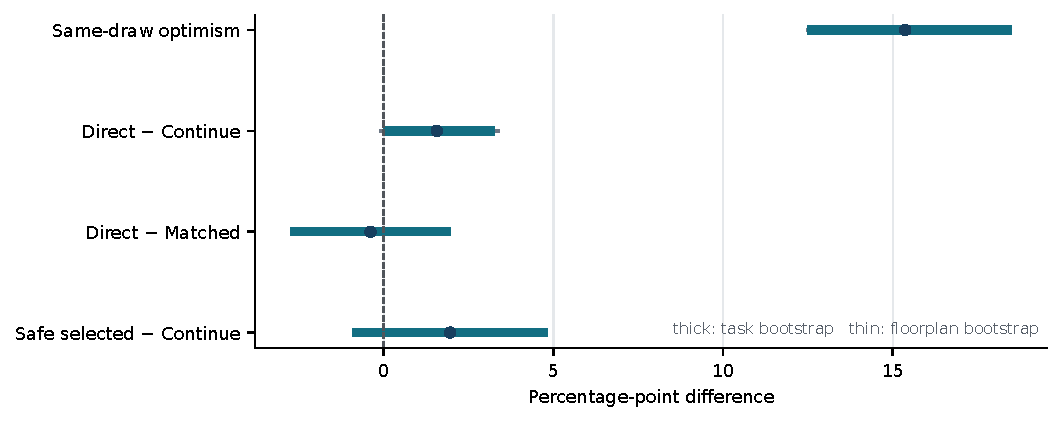
\includegraphics[width=\linewidth]{figures/policy-effects.pdf}
\caption{Confirmation effects on ALFWorld. Dots show planned-task means; thick and thin intervals show task- and floorplan-bootstrap 95\% intervals. Reported adjusted $p$ values use the prespecified group sign-flip tests and Holm correction.}
\label{fig:effects}
\end{figure}


\begin{figure}[ht]
\centering
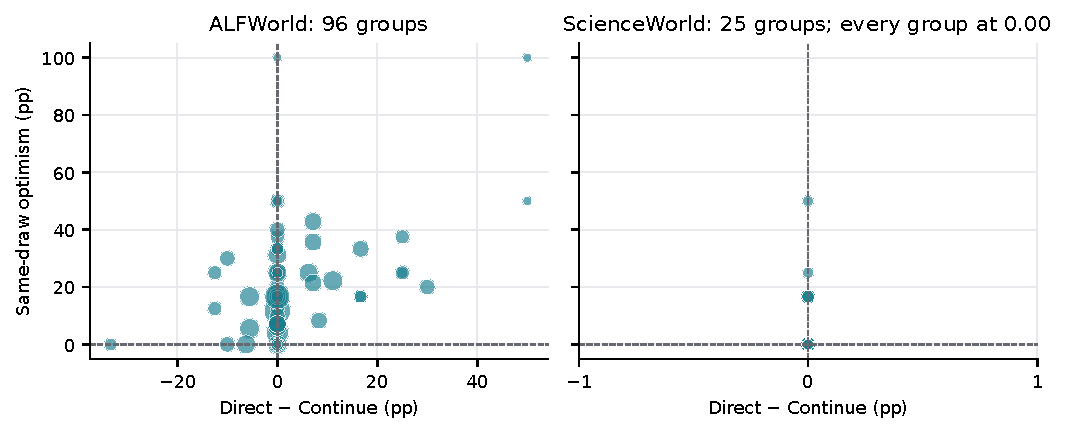
\includegraphics[width=\linewidth]{figures/group-results.pdf}
\caption{Group-level measurement and policy effects. Each point is a complete floorplan or task-family group; area is proportional to its task count. Vertical position is same-draw optimism and horizontal position is Direct minus Continue. Dashed lines mark zero.}
\label{fig:groups}
\end{figure}



\begin{table}[ht]
\caption{All ALFWorld contrasts. Values are percentage points. Holm adjustment applies only to the first two rows and the same-draw diagnostic in the text.}
\label{tab:alfworld-contrasts}
\centering
\scriptsize
\begin{tabular}{@{}lrrrrr@{}}
\toprule
Contrast & Mean & Task 95\% & Group 95\% & Group $p$ & Holm $p$ \\
\midrule
Direct $-$ Continue & 1.56 & [0.00, 3.26] & [\ensuremath{-0.12}, 3.41] & 0.1048 & 0.2096 \\
Direct $-$ Matched & \ensuremath{-0.39} & [\ensuremath{-2.73}, 1.95] & [\ensuremath{-2.26}, 1.57] & 0.7927 & 0.7927 \\
Direct $-$ Arm outcome & 0.39 & [\ensuremath{-2.21}, 2.99] & [\ensuremath{-1.82}, 2.64] & 0.8228 & -- \\
Direct $-$ Best fixed & \ensuremath{-0.91} & [\ensuremath{-3.39}, 1.56] & [\ensuremath{-3.09}, 1.31] & 0.4881 & -- \\
Safe selected $-$ Continue & 1.95 & [\ensuremath{-0.91}, 4.82] & [\ensuremath{-0.38}, 4.26] & 0.1311 & -- \\
\bottomrule
\end{tabular}
\end{table}

\begin{table}[ht]
\caption{All ScienceWorld contrasts, retained as unadjusted boundary analyses. Values are percentage points.}
\label{tab:scienceworld-contrasts}
\centering
\scriptsize
\begin{tabular}{@{}lrrrrr@{}}
\toprule
Contrast & Mean & Task 95\% & Group 95\% & Group $p$ & Holm $p$ \\
\midrule
Direct $-$ Continue & 0.00 & [0.00, 0.00] & [0.00, 0.00] & 1.0000 & -- \\
Direct $-$ Matched & 5.26 & [\ensuremath{-0.88}, 12.28] & [\ensuremath{-0.81}, 11.86] & 0.1860 & -- \\
Direct $-$ Arm outcome & 0.00 & [\ensuremath{-5.26}, 5.26] & [\ensuremath{-4.17}, 4.39] & 1.0000 & -- \\
Direct $-$ Best fixed & 0.00 & [\ensuremath{-5.26}, 5.26] & [\ensuremath{-4.17}, 4.39] & 1.0000 & -- \\
Safe selected $-$ Continue & \ensuremath{-5.26} & [\ensuremath{-12.28}, 0.88] & [\ensuremath{-11.86}, 0.81] & 0.1860 & -- \\
\bottomrule
\end{tabular}
\end{table}

ALFWorld same-draw optimism is 15.36 percentage points with task-bootstrap interval [12.50, 18.49], group-bootstrap interval [12.46, 18.30], raw group sign-flip $p=<10^{-4}$, and Holm-adjusted $p=<10^{-4}$. These preregistered $p$ values are retained for audit; the nonnegative gap makes their symmetric null scientifically narrow, and they are not tests of intervention benefit. ScienceWorld optimism is 5.26 percentage points with task-family-bootstrap interval [1.69, 10.00] and unadjusted group sign-flip $p=0.0632$.

\begin{table}[ht]
\caption{Mean selected-suffix cost per planned task. Structural early terminations have zero suffix cost.}
\label{tab:costs}
\centering
\small
\begin{tabular}{@{}llrrrr@{}}
\toprule
Domain & Policy & Requests & Input tokens & Output tokens & Client seconds \\
\midrule
\multirow{6}{*}{ALFWorld} & Continue & 28.1 & 43557 & 1508 & 64.9 \\
 & Best fixed & 27.5 & 43237 & 1468 & 63.2 \\
 & Direct & 27.4 & 42560 & 1470 & 63.4 \\
 & Arm outcome & 27.7 & 43559 & 1481 & 63.8 \\
 & Matched & 27.7 & 43459 & 1487 & 64.1 \\
 & Safe selected & 27.7 & 43459 & 1487 & 64.1 \\
\midrule
\multirow{6}{*}{ScienceWorld} & Continue & 47.7 & 177369 & 2836 & 124.6 \\
 & Best fixed & 48.3 & 193820 & 2837 & 126.5 \\
 & Direct & 47.7 & 178377 & 2847 & 125.3 \\
 & Arm outcome & 48.3 & 193820 & 2837 & 126.5 \\
 & Matched & 52.8 & 199333 & 3139 & 138.0 \\
 & Safe selected & 52.8 & 199333 & 3139 & 138.0 \\
\bottomrule
\end{tabular}
\end{table}

Across baseline, arm, and retained attempt records, the episode ledger contains 127,213 model requests, 253,758,979 input tokens, 6,921,686 output tokens, and 301,110.6 client-seconds. It records 561 failed requests and 561 requests with unknown token usage. The separate GPU lease ledger charges model loading, qualification probes, generation, idle occupancy, failures, and cleanup.


We also raised learner capacity directly, on development data and before any test prediction. Nested honest out-of-fold utility is 29.47\% for the frozen forest at the scheduled point and 50.69\% at the triggered one; gradient boosting, appended 0.6B language-model embeddings of the prefix, and their combination each score lower at both (29.27, 29.10, 28.84 and 49.46, 50.29, 50.15). What the prefix carries at a decision point, not the model class, decides what a learner recovers. The same grid traces the trade-off between expected gain and the significance of that gain. Across the frozen candidate set the development improvement over continuation reaches 3.09 points and the paired $z$ statistic reaches 2.60; the configuration the pre-registered utility criterion selected is the one attaining that maximum, at 2.94 points over 11.5\% discordant tasks. The frozen operating point is the most certifiable one the menu offers, not the most aggressive.

\begin{table}[ht]
\caption{Complete policy census under both checkpoint rules. Success uses every planned task; firing is over eligible prefixes; recoveries and disruptions count draw-level comparisons with continuation.}
\label{tab:r2-policies}
\centering
\small
\begin{tabular}{@{}llrrrr@{}}
\toprule
Rule & Policy & Success (\%) & Fire (\%) & Recover & Disrupt \\
\midrule
\multirow{10}{*}{Event-triggered} & Continue & 54.97 & 0.0 & 0 & 0 \\
 & Best fixed & 54.30 & 100.0 & 105 & 113 \\
 & Direct & 56.24 & 54.1 & 62 & 47 \\
 & Arm outcome & 54.81 & 10.1 & 10 & 12 \\
 & Matched & 55.06 & 0.8 & 3 & 2 \\
 & Comparison-only & 55.48 & 54.9 & 60 & 54 \\
 & Failure risk & 54.38 & 81.9 & 94 & 101 \\
 & Lower bound & 54.97 & 0.0 & 0 & 0 \\
 & Cross-draw & 56.24 & 40.0 & 52 & 37 \\
 & Safe selected & 56.24 & 40.0 & 52 & 37 \\
\midrule
\multirow{10}{*}{Scheduled} & Continue & 54.72 & 0.0 & 0 & 0 \\
 & Best fixed & 57.50 & 100.0 & 140 & 107 \\
 & Direct & 55.65 & 35.7 & 52 & 41 \\
 & Arm outcome & 54.72 & 2.8 & 2 & 2 \\
 & Matched & 54.72 & 0.4 & 0 & 0 \\
 & Comparison-only & 55.99 & 37.8 & 49 & 34 \\
 & Failure risk & 58.43 & 86.1 & 130 & 86 \\
 & Lower bound & 54.72 & 0.0 & 0 & 0 \\
 & Cross-draw & 55.23 & 26.3 & 37 & 31 \\
 & Safe selected & 55.23 & 26.3 & 37 & 31 \\
\bottomrule
\end{tabular}
\end{table}

\begin{table}[ht]
\caption{Complete contrast census on the event-triggered panel. Intervals are 95\% task and floorplan bootstraps; adjusted values apply Holm correction within the pre-registered family.}
\label{tab:r2-contrasts}
\centering
\small
\begin{tabular}{@{}lrrrrr@{}}
\toprule
Contrast & Estimate (pp) & Task 95\% & Group 95\% & Raw $p$ & Adjusted $p$ \\
\midrule
Cross-draw $-$ Continue & 1.26 & [$-$0.51, 3.04] & [$-$0.35, 2.83] & 0.1579 & 0.1579 \\
Cross-draw $-$ Best fixed & 1.94 & [$-$0.17, 4.05] & [$-$0.17, 4.17] & 0.0855 & -- \\
Cross-draw $-$ Direct & 0.00 & [$-$1.43, 1.43] & [$-$1.48, 1.57] & 1.0000 & -- \\
Cross-draw $-$ Arm outcome & 1.43 & [$-$0.17, 3.04] & [$-$0.09, 2.94] & 0.0957 & -- \\
Cross-draw $-$ Matched & 1.18 & [$-$0.51, 2.87] & [$-$0.35, 2.68] & 0.1671 & -- \\
Cross-draw $-$ Comparison-only & 0.76 & [$-$0.93, 2.36] & [$-$0.82, 2.43] & 0.4226 & -- \\
Cross-draw $-$ Failure risk & 1.85 & [$-$0.25, 3.88] & [$-$0.24, 4.05] & 0.1001 & -- \\
Cross-draw $-$ Lower bound & 1.26 & [$-$0.51, 3.04] & [$-$0.35, 2.83] & 0.1579 & -- \\
Direct $-$ Continue & 1.26 & [$-$0.59, 3.20] & [$-$0.79, 3.15] & 0.2630 & -- \\
Comparison-only $-$ Continue & 0.51 & [$-$1.43, 2.45] & [$-$1.60, 2.50] & 0.6892 & -- \\
Failure risk $-$ Continue & $-$0.59 & [$-$2.95, 1.77] & [$-$3.45, 2.11] & 0.7244 & -- \\
Lower bound $-$ Continue & 0.00 & [0.00, 0.00] & [0.00, 0.00] & 1.0000 & -- \\
Safe selected $-$ Continue & 1.26 & [$-$0.51, 3.04] & [$-$0.35, 2.83] & 0.1579 & -- \\
\bottomrule
\end{tabular}
\end{table}

\begin{table}[ht]
\caption{Pre-outcome lineage for the event-triggered study. Both checkpoint rules run the same 288 identities; predictions were frozen after baselines and before any arm outcome.}
\label{tab:r2-lineage}
\centering
\small
\begin{tabular}{@{}lp{0.55\linewidth}@{}}
\toprule
Object & Frozen identifier \\
\midrule
Event-triggered eligible prefixes & 497 \\
Event-triggered prefix digest & \texttt{d20c439a...ba0775} \\
Event-triggered prediction digest & \texttt{738b1ff3...8ec801} \\
Scheduled eligible prefixes & 540 \\
Scheduled prefix digest & \texttt{02fc748b...332f88} \\
Scheduled prediction digest & \texttt{a869e454...1e3d43} \\
\bottomrule
\end{tabular}
\end{table}


\section{Historical and exploratory evidence}
\label{app:historical}

Earlier work motivated the new confirmation but does not enter its multiplicity family. On a 134-game official unseen ALFWorld panel with a different actor interface, the prior repeated-branch learner reached 68.16\% against 69.40\% for continuation, a difference of $-1.24$ percentage points with task-bootstrap interval $[-4.98,2.24]$ and $p=0.5946$. Same-arm mismatches ranged from 8.25\% to 12.06\%, and the same-draw sample oracle exceeded a fresh-replica evaluation by 7.94 points. A four-stratum retrospective direct-benefit reanalysis averaged 30.14\%, compared with 32.62\% for continuation and 28.92\% for the repeated-outcome policy. These records motivated independent continuation evaluation and the direct target comparison; they do not confirm either new hypothesis.

The native-interface follow-up and its demonstration ablation are reported only as actor-side exploratory analyses. Changing thinking mode, output cap, and demonstration use together produced 80.60\% versus 70.90\% in one paired 134-task draw. A later conditional ablation held thinking and cap fixed: including two released demonstrations produced 116/134 successes (86.57\%) versus 107/134 (79.85\%), a $+6.72$ percentage-point estimate with task-bootstrap interval $[-0.75,14.18]$ and two-sided sign-flip $p=0.1087$. Excluding one scene reversed the latter estimate to $-3.51$ points. Neither result is pooled with confirmation, establishes a controller effect, or supports a state-of-the-art claim.

A separate 27B experiment is retained as a systems result. On its internal reserved panel, the plain 27B actor scored 131/160 (81.88\%) against 76/160 (47.50\%) for an 8B self-check system; the paired difference was $+34.38$ percentage points with a prespecified two-sided 97.5\% cluster-$t$ interval $[24.20,44.55]$, whose lower limit is the one-sided 98.75\% bound recorded for that systems check; every other interval in this paper is reported at 95\%. The systems differ in model, policy, filtering, and decoder stream, and 49 of 64 confirmation floorplans had appeared in historical tasks. On the historically exposed 134-task public ALFWorld frame, the plain and self-check 27B systems both scored 108/134. These results establish neither an isolated parameter-count effect nor a controller advance and are not pooled with confirmation. A separate internal retrieval study on an unrelated corpus is outside this paper.

A temperature ablation runs the same checkpoint rule, menu, and draw count twice on 91 shared identity-disjoint ALFWorld tasks, once at the frozen sampling temperature of 0.7 and once at 1.0. It separates the diagnostic from the knob usually assumed to drive it. At 0.7 the mean per-task outcome variance is 0.0936 and the same-draw gap is 21.98 percentage points; at 1.0 the variance is 0.0796 and the gap is 16.48 points. Raising the temperature did not raise the variance on these tasks, and the gap moves with it. Temperature is therefore an indirect and non-monotone handle: what the diagnostic follows is the variance of the continuation outcome itself, which the profile in the main text measures directly within a single panel. A domain whose tools or simulated users inject randomness of their own raises that variance and so raises the gap, which is the sense in which the estimates here are a lower reference for such settings. This ablation is exploratory: its panel is small, it was generated after the confirmation panels, and it enters no confirmatory family.


The variance profile reported in Section~\ref{sec:analysis} and this ablation answer the same question from two directions: within one panel the diagnostic rises with per-task outcome variance, and across a matched pair of panels it moves with the sampling temperature that produces that variance. The released evidence index preserves those boundaries rather than using favorable actor or domain subsets to replace the frozen confirmation.

\section{Reproduction}
\label{app:repro}

The anonymous supplement contains the exact ICLR source, panel manifests, frozen prefix features and actions, controller manifests, raw confirmation records, analysis environment lock, tests, evaluator, rendering program, and artifact manifest. Model weights and benchmark installations are excluded. Analysis and paper regeneration require no GPU.

\begin{verbatim}
uv venv --python 3.12 .venv
uv sync --frozen
.venv/bin/python -m pytest -q
mv artifacts/confirmation artifacts/confirmation.release
.venv/bin/python controller/evaluate_confirmation.py \
  --config configs/independent-panel/panel-shard0.json \
  --config configs/independent-panel/panel-shard1.json \
  --config configs/independent-panel/panel-shard2.json \
  --config configs/independent-panel/panel-shard3.json \
  --config configs/independent-panel/panel-shard4.json \
  --config configs/independent-panel/panel-shard5.json \
  --config configs/independent-panel/panel-shard6.json \
  --config configs/independent-panel/panel-shard7.json \
  --raw raw \
  --predictions artifacts/prediction-freeze/predictions.json \
  --prediction-freeze \
    artifacts/prediction-freeze/prediction-freeze.json \
  --out artifacts/confirmation
.venv/bin/python paper/build_assets.py
cd paper
mkdir -p build
pdflatex -interaction=nonstopmode -halt-on-error \
  -output-directory=build main.tex
BIBINPUTS=.: BSTINPUTS=.: bibtex build/main
pdflatex -interaction=nonstopmode -halt-on-error \
  -output-directory=build main.tex
pdflatex -interaction=nonstopmode -halt-on-error \
  -output-directory=build main.tex
cd ..
.venv/bin/python tools/verify_artifacts.py --supplement \
  ../intervene-or-continue-iclr2027-supplement.zip
\end{verbatim}

The second study reuses the same programs. Its panels are frozen with \texttt{extension/freeze\_panel.py} under \texttt{--checkpoint-rule event} and \texttt{--checkpoint-rule scheduled} on one shared set of identities, its development rows are built by \texttt{extension/analysis.py}, its three learners are fitted by \texttt{extension/policies.py}, \texttt{controller/fit\_direct.py}, and \texttt{controller/fit\_cross\_draw.py}, its predictions are frozen by \texttt{controller/freeze\_predictions.py} with the cross-draw bundle attached, and its results are produced by \texttt{controller/evaluate\_confirmation.py} with \texttt{--primary CROSS\_DRAW\_vs\_CONTINUE --primary CROSS\_DRAW\_vs\_BEST\_FIXED}. Tables and figures for both studies regenerate through \texttt{paper/build\_assets.py} and \texttt{paper/build\_assets\_r2.py}.

Inference reproduction additionally requires ALFWorld 0.4.2, TextWorld 1.7.0, ScienceWorld 1.3.0, the recorded Qwen3-8B revision, and the content-addressed serving image. Each GPU worker receives one panel shard and a unique port. A bounded coordinator enforces a 72,000 H100 GPU-second actual-or-reserved occupancy cap; closed leases return unused reservation headroom. The immutable ledger records 47,876.7 charged H100 GPU-seconds across 26 closed leases. Exact request seeds are derived from task identity, arm, draw, and request index. New stochastic generations are replications and must not overwrite the released outcomes.

The supplement's verification program checks the source commit, all protected input hashes, complete task and cell counts, task/fold disjointness, action visibility, panel exclusions, prediction freeze, recomputed result JSON, figure inputs, page limit, unresolved references, anonymous strings, and final archive digest. Absolute execution paths and private repository ownership are replaced by symbolic roots in the anonymous archive; scientific identifiers and file-content digests are unchanged.

\section{AI assistance and author responsibilities}
\label{app:ai}

AI tools were used for literature discovery through alphaXiv, code drafting, statistical and manuscript review, LaTeX drafting, copyediting, and format inspection. Manuscript structure was checked against five pre-2024 ICLR papers on grounded language agents and prompting, read from their arXiv sources: BabyAI, ALFWorld, self-consistency, least-to-most prompting, and ReAct. The released audit records their abstract and section lengths, their float conventions, a per-section profile of sentence length, first-person density and hedging, and a vocabulary comparison in which the reference papers cover one another at 79 to 89 percent of tokens while this manuscript reaches 71 percent. The shortfall is carried by the study's own objects, which are retained; no word was substituted to move that statistic, and no perplexity target or author imitation was used. They were not treated as authors. The pre-outcome commits and immutable result evaluator separate assistance during design from outcome-conditioned reporting. The complete result census, adverse evidence, source links, and assistance ledger are provided for audit. Human authors remain responsible for checking claims, citations, authorship, conflicts, affiliations, eligibility, disclosure categories, and the final submission.


\end{document}
